\chapter{General Discussion to Configuration Interation Methods}
%
%
%
%
\section{The Limitation of The HF Theory}
%
% does not include the correlation effects how to understand the
% correlation effects, in the pictured way Pauli effects and
% correlation effects
%
On the base of single electron approximation, the Hatree-Fock theory
succeeds in making good approximation to the schrodinger equation.  In
a sufficiently large basis sets, the HF wave function can account for
$99$ percent of the total energy. However, the remaining $1$ percent
is always fatal in describing chemical phenomenon.

What does the error in HF theory come from? Generally to say, this is
due to the single electron approximation. As the quantum law declares
that there's correlation between quantum particles (electron is surely
included in), it's impossible for the quantum particles to move in an
irrelevant way. More specifically, here we can give a naive but easily
understood description.

As a result of HF calculation, the electrons are grouped in pair to
reside in the HF orbitals, starting from the orbital with lowest
energy. Thus, for a closed shell system, each orbital are taken by
pair of electrons with opposite spin. The spatial overlap between such
pair of electrons is exactly one, while the overlap between two
electrons belonging to different orbitals is exactly zero because of
the orthogonality.

Naively to say, this can not be true. For electrons are quantized,
it's impossible for two pair of electrons to share exactly the same
orbital, only different in spin. When one electron moves, the other
must be "correlated". This holds true for electrons in different
orbitals, too. Their moving is correlated so that the orthogonality is
only a kind of approximation.

The difference between the exact ground state energy and the HF energy
(under the non relativistic condition and the Born-Oppenheimer
approximation) is called \textbf{electron correlation energy}. To some
extent, such correlation is called coulomb correlation, it arises
between electrons in opposite spin among orbitals, for the pauli
principle has the consequence that there is no intraorbital
correlation from electron pairs with same spin. The correlation
attributed to the pauli principle, is called Fermi correlation; which
has been exactly contained in the HF theory.

If we want to contain the correlation energy, we have to step into the
CI (configuration interaction ) method.

%%%%%%%%%%%%%%%%%%%%%%%%%%%%%%%%%%%%%%%%%%%%%%%%%%%%%%%
\section{How to Form The CI Wave Functions}\label{CI2}
%
% 1 requirement to form the wave functions 2 the requirement for the
% basis functions 3 use the permutation operator to express the
% permutation process to the orbital 4 get the determinant form
%
the first question in the CI method, is that how to form the wave
functions. Firstly we note that such wave functions should satisfy two
points:
\begin{itemize}
\item wave functions should be arisen from a complete set of basis
  functions
\item wave functions should satisfy the anti-symmetric properties
  while exchanging electrons
\end{itemize}

In general, we can have many ways to realize such construction
satisfying the requirements above. For example, the linear combination
of plane waves. However, in quantum chemistry, we always use the
spin-orbitals as the basis functions, that is:
\begin{equation}\label{}
  \varphi_{A}(r,s), \varphi_{B}(r,s), \cdots, \varphi_{X}(r,s)
\end{equation}
Here on each orbital there may has electron residing on it (which is
called occupied orbital); or no electrons residing on it (so called
virtual orbital). The total $N$ electrons are considered to be
distributing over such set of basis functions, each one is orthogonal
with the other and satisfying the normalized condition.  Here we note
that generally we do not care how the orbitals we can get, but usually
they are gotten from HF calculation; but here we only consider the
general character of the basis functions, which is required to be
complete, orthogonal and normalized.

Then the question is: how to build the wave functions based on such
series of $\varphi_{k}$ ($k = A, B, \cdots, X$)?

First, generally we can the total wave function of $\Phi$ expressed
as:
\begin{equation}\label{}
  \Phi = \sum_{A,B, \cdots, X}C_{AB\cdots
    X}\varphi_{A}\varphi_{B}\cdots\varphi_{X}
\end{equation}
Then, for a given set of spin-orbitals, that is the $A, B, \cdots, X$
are fixed to be certain; we can see that the electrons label are
totally arbitrary. The electron $1$ can be considered to be setting on
the $\varphi_{A}$, or $\varphi_{B}$; which does not change the whole
wave function of $\Phi$.

Therefore, we can use some permutation operator of $\hat{P}$ (more
discussion can see the quantum mechanics part, the chapter related to
the identity particle), which is used to change all the $N$ electrons
among the $A, B, \cdots, X$ orbitals:
\begin{equation}\label{}
  \hat{P} = \prod_{1\leq i<j\leq N}\hat{P}_{ij}
\end{equation}
Here the $\hat{P}_{ij}$ is the exchange operator for exchanging the
electron $i$ and $j$. Hence, we can have:
\begin{align}\label{}
  \hat{P}\Phi &= (-1)^{P}\Phi \Rightarrow \nonumber \\
  \Phi &=\sum_{A,B, \cdots, X}C_{AB\cdots
    X}(-1)^{-P}\hat{P}\{\varphi_{A}\varphi_{B}\cdots\varphi_{X}\}
  \nonumber \\
  &=\sum_{A,B, \cdots, X}C_{AB\cdots
    X}(-1)^{P}\hat{P}\{\varphi_{A}\varphi_{B}\cdots\varphi_{X}\}
  \nonumber \\
\end{align}
Here from the definition of $P$ we surely have $(-1)^{-P} = (-1)^{P}$.

From mathematics, it's clear to know that such permutation can be
equivalently expressed as determinant, thus we finally have:
\begin{equation}\label{CIeq:26}
  \Phi = \sum_{A,B, \cdots, X}C_{AB\cdots X}
  \frac{1}{\sqrt{N!}}\begin{vmatrix}
    \varphi_{A}(1) & \varphi_{A}(2) & \cdots & \varphi_{A}(n) \\
    \varphi_{B}(1) & \varphi_{B}(2) & \cdots & \varphi_{B}(n) \\
    \cdots & \cdots & \cdots & \cdots \\
    \varphi_{X}(1) & \varphi_{X}(2) & \cdots & \varphi_{X}(n) \\
  \end{vmatrix}
\end{equation}
Therefore, by changing the $A,B, \cdots, X$, for example; to change
the $A$ orbital into the $Y$ orbital; we will get another
determinant. Then their linear combination is finally forming the wave
functions.

Finally, we note that the form of (\ref{CIeq:26}) is general. It's not
only for HF orbitals, but also for any other basis functions used to
constructing the CI wave function. From this concept, we can naturally
have the impression about the root determinant and the exciting
determinants; as what will be mentioned below.


%%%%%%%%%%%%%%%%%%%%%%%%%%%%%%%%%%%%%%%%%%%%%%%%%%%%%%%%
\section{Basic Idea in CI Algorithm}
%
% 1 address the idea of the variational process 2 introduce the
% concept of configuration
%
%
The main idea for the CI, is very simple and straightforward; that is
only based on the variational principle.

The variational principle states that if we have a set of approximate
wave function (usually it's the determinants of what we have just
talked about), which is complete, orthogonal and normalized; the
linear combination of the approximate wave function can have an energy
which is above or equal to the exact energy. In the following content,
we will give a demonstration of the theory.

We can use the variational principle in this way: first construct an
approximate wave function of $\Psi$, which satisfies the condition of
the exact wave function, but has some flexible parameters as $a_{1},
a_{2}, \cdots, a_{l}$; so the above variational principle can write
as:
\begin{eqnarray} \label{CIeq:1}
  % \nonumber to remove numbering (before each equation)
  E(a_{1}, a_{2}, \cdots, a_{l}) &=&  \frac{\langle \Psi|\hat{H}| \Psi
    \rangle} {\langle \Psi|\Psi \rangle} \nonumber \\
  & \geq & E_{0}
\end{eqnarray}

Then we can properly choose the flexible parameters of $a_{1}, a_{2},
\cdots, a_{l}$ so that to make $E(a_{1}, a_{2}, \cdots, a_{l})$ is a
minimum. Here the minimum energy is as the upper boundary of the true
energy, and the difference between them depends on the quality of the
approximate wave function we use. The set of flexible parameters are
required as:
\begin{equation}\label{CIeq:2}
  \frac{\partial E(a_{1}, a_{2}, \cdots, a_{l})}{\partial a_{k}} = 0
  (k= 1,2, \cdots, l)
\end{equation}

In CI calculation, we always choose the linear combination of the
slater determinants as the approximate wave function, each of the the
approximate slater determinant is called "configuration".

The slater determinants are formed from a HF calculation. After the HF
calculation, we can get a set of HF occupied orbitals and virtual
orbitals. By firing the electrons on the occupied orbital onto the
virtual orbital, we can get the excited slater determinant. So sorted
by the electrons fired up onto the virtual orbitals, we have singly,
doubly, triply etc. excited relative to the ground HF determinant. the
illustration of the excited determinants can see the figure of
(\ref{CI1}).Their combination can be written as:
\begin{equation}\label{CIeq:3}
  \Psi_{CI} = a_{0}\Psi_{HF} + \sum _{S}a_{S}\Psi_{S} + \sum
  _{D}a_{D}\Psi_{D} + \sum _{T}a_{T}\Psi_{T} + \cdots
\end{equation}

\begin{figure}[htp]
  \begin{center}
    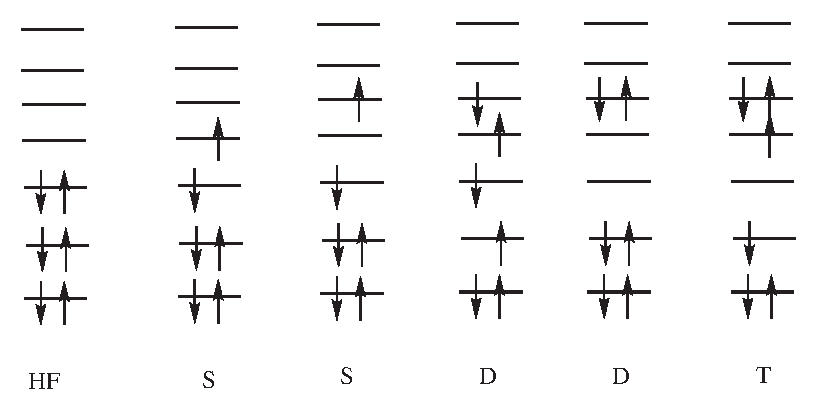
\includegraphics[scale=1.0]{ci.eps}\label{CI1}
    \caption{illustration of the excited determinants}
  \end{center}
\end{figure}

Before the deduction of the variational principle, it's appropriate
for us to make an outline of this method, and specify some important
points.

In the CI methods, first we run HF calculation, then we form the
configurations; finally we can get the CI wave function by energy
minimization. Thus this method is two-dimensional, the size of HF
orbitals (which is determined by the size of the basis sets), and the
number of determinants; are the two loosely independent factors that
influencing the result of the CI calculation.

Therefore, the larger of the basis sets, and the larger number of the
slater determinants; the more better result that the CI calculation
can achieve.

It's worthy to note here, that the CI method includes the exact Fermi
correlation, which is the same as the HF theory.

This point is important, but very easy to prove. As shown in the
(\ref{CIeq:3}), we can write the CI wave function as:
\begin{equation}\label{}
  \Phi_{CI} (1,2,\cdots, n) = \sum _{i}a_{i}\Psi_{i} (1,2,\cdots, n)
\end{equation}
If we interchange electron k,l in the $\Psi_{i} (1,2, \cdots, k,l,
\cdots, n)$ to make it become $\Psi_{i} (1,2, \cdots, l,k, \cdots, n)$
for all the determinants $i=1,2, \cdots, n$; that leads to the
$-\Psi_{CI}(1,2,\cdots, n)$; which is equivalent to interchange
electrons k,l in the $\Psi_{CI}$.


%%%%%%%%%%%%%%%%%%%%%%%%%%%%%%%%%%%%%%%%%%%%%%%%%%
\section{Variational Process in CI}
%
%
%
%
So now we can go to prove the variational process used in the CI
algorithm. This general derivation is taken from Tang's
book\cite{aoqingTang}, and I favor this demonstration for it's
clearness and simplicity. Here in the following content, the $\Phi$ is
designated as the CI wave function, and the $\Psi$ is designated as
the slater determinant; we do so just because in the HF chapter the
$\Psi$ is designated as the HF wave function (the root slater
determinant).

Based on the variational principle, we can express any CI wave
function by this way:
\begin{equation}\label{CIeq:4}
  \Phi = \sum_{j}c_{j}\Psi_{j}
\end{equation}
So by inserting this expression into the schrodinger function, we
have:
\begin{equation}\label{CIeq:5}
  \sum_{j}c_{j}\hat{H}\Psi_{j} = E\sum_{j}c_{j}\Psi_{j}
\end{equation}

By multiplying the left bra of $\langle\Phi|$, which is actually
expressed as $\sum_{i}c_{i}^{*}\Psi_{i}$; we have:
\begin{equation}\label{CIeq:6}
  \sum\limits_{i}\sum\limits_{j}c_{i}^{*}c_{j}\langle\Psi_{i}|\hat{H}|\Psi_{j}\rangle
  =E\sum\limits_{i}\sum\limits_{j}c_{i}^{*}c_{j}\langle\Psi_{i}|\Psi_{j}\rangle
\end{equation}

Which finally yields:
\begin{equation}\label{CIeq:7}
  E=\frac{\sum_{i}\sum_{j}c_{i}^{*}c_{j}\langle\Psi_{i}|\hat{H}|\Psi_{j}\rangle}
  {\sum_{i}\sum_{j}c_{i}^{*}c_{j}\langle\Psi_{i}|\Psi_{j}\rangle}
\end{equation}

as we make a bit change to $c_{i}^{*}$, make it to $c_{i}^{*}+\delta
c_{i}^{*}$, here the right ket of $|\Phi\rangle$ is also changed.
Hence the $E$ is changed to the $E+\delta E$; so we have:
\begin{equation} \label{CIeq:8} E+\delta E =
  \frac{\sum_{i}\sum_{j}(c_{i}^{*}+\delta c_{i}^{*})(c_{j}+\delta
    c_{j}) \langle\Psi_{i}|\hat{H}|\Psi_{j}\rangle}
  {\sum_{i}\sum_{j}(c_{i}^{*}+\delta c_{i}^{*})(c_{j}+\delta c_{j})
    \langle\Psi_{i}|\Psi_{j}\rangle}
\end{equation}

The expression above is a bit wordy, so we rewrite it into a
compressed form:
\begin{equation}\label{CIeq:9}
  E+\delta E = \frac{(C+\delta C)^{*}H(C+\delta C)}{(C+\delta C)^{*}M(C+\delta C)}
\end{equation}
In the expression above, the $C$ is the compression of $\sum c_{i}$,
and $H$ is the matrix of $\langle\Psi_{i}|\hat{H}|\Psi_{j}\rangle$;
that is:
\begin{equation}\label{CIeq:10}
  \left [ \begin{array}{cccc}
      \langle\Psi_{1}|\hat{H}|\Psi_{1}\rangle & \langle\Psi_{1}|\hat{H}|\Psi_{2}\rangle & \cdots & \langle\Psi_{1}|\hat{H}|\Psi_{n}\rangle \\
      \langle\Psi_{2}|\hat{H}|\Psi_{1}\rangle & \langle\Psi_{2}|\hat{H}|\Psi_{2}\rangle & \cdots & \langle\Psi_{2}|\hat{H}|\Psi_{n}\rangle \\
      \cdots & \cdots & \cdots & \cdots                                  \\
      \langle\Psi_{n}|\hat{H}|\Psi_{1}\rangle & \langle\Psi_{n}|\hat{H}|\Psi_{2}\rangle & \cdots & \langle\Psi_{n}|\hat{H}|\Psi_{n}\rangle
    \end{array} \right ]
\end{equation}

the $M$ is similar to the $H$, which has no $\hat{H}$. So as the
(\ref{CIeq:8}) is compressed into the matrix form, the meaning is more
clear.

From (\ref{CIeq:9}) we have:
\begin{equation}\label{CIeq:11}
  E + \delta E = \frac{C^{*}HC + \delta C^{*}HC + C^{*}H \delta C + \delta C^{*}H \delta C }
  {C^{*}MC + \delta C^{*}MC + C^{*}M \delta C + \delta C^{*}M \delta C}
\end{equation}
We omit all the second order infinitesimal, and we have:
\begin{equation}\label{CIeq:12}
  E + \delta E = \frac{1}{C^{*}MC} \frac{C^{*}HC + \delta C^{*}HC + C^{*}H \delta C }
  { 1+ \frac{\delta C^{*}MC + C^{*}M \delta C}{C^{*}MC}}
\end{equation}
Furthermore to expand this math expression to infinite series and omit
the second order infinitesimal, we can write:
\begin{equation}\label{CIeq:13}
  \frac{1}{ 1+ \frac{\delta C^{*}MC + C^{*}M \delta C}{C^{*}MC} } = 1
  - \frac{\delta C^{*}MC + C^{*}M \delta C}{C^{*}MC}
\end{equation}


So we have:
\begin{equation}\label{CIeq:14}
  E + \delta E = \frac{C^{*}HC + \delta C^{*}HC + C^{*}H \delta
    C}{C^{*}MC} * (1 - \frac{\delta C^{*}MC + C^{*}M \delta C}{C^{*}MC})
\end{equation}

By remembering that $E=\frac{C^{*}HC}{C^{*}MC}$, and also omit the
second order infinitesimal; we finally have this expression:
\begin{equation}\label{CIeq:15}
  \delta C^{*}HC + C^{*}H \delta C - E(\delta C^{*}MC + C^{*}M \delta
  C) = 0
\end{equation}
Here we drop the denominator for the $C^{*}MC$ is always larger than
0.

From the expression above, by separating the two different
infinitesimal, which are $\delta C^{*}$ and $\delta C$; we can get
that:
\begin{eqnarray}\label{CIeq:16}
  % \nonumber to remove numbering (before each equation)
  \delta C^{*}(HC-EMC)  &=& 0 \nonumber \\
  (C^{*}H-EC^{*}M)\delta C&=& 0
\end{eqnarray}
And actually they are the same. We can transpose one to the another.
So finally we get the answer:
\begin{equation}\label{CIeq:17}
  HC=EMC
\end{equation}

If we select the Slater determinants as the reference for expansion, then it's
easy to know that:
\begin{equation}
 M_{ij} = \delta_{ij} 
\end{equation}
so we have $HC=EC$. By diagonal we can the energy.

%%%%%%%%%%%%%%%%%%%%%%%%%%%%%%%%%%%%%%%%%%%%%%%%%%%%%%
\section{CI Matrix Elements}
After setting up the general algorithm of the CI, next step we are
going to introduce some simple rules to evaluate its matrix
elements. Here the evaluation is only related to the spatial part of
the orbital, so only the singly excited determinant of S, and D, T,
etc. are concerned into this part.

%%%%%%%%%%%%%%%%%%%%%%%%%%%%%%%%%%%%%%%%%%%%%%%%%%%%%%
\subsection{Brillouin's Theorem}
%
% simple statement about this theorem
%
Brillouin's theorem is a simple and direct result of HF theory, it
states that the overlap between the ground state configuration of
$|\Psi \rangle$ and the singly excited determinant of $|\Psi^{r}
\rangle$ (in which one of occupied orbital of $\varphi_{s}$ has been
replaced by an unoccupied orbital of $\varphi_{r}$, so we designated
this configuration as $|\Psi^{r} \rangle$) is zero, that means to
include the singly excited determinant into the root determinant has
no contribution to the ground state energy.

So we can prove it. Suppose that the CI wave function is written as:
$|\Phi \rangle= a_{0}|\Psi \rangle+ a_{1}|\Psi^{r}\rangle$, here we
have the $|\Psi \rangle$ just as the determinant we use in the
(\ref{HFTeq:20})(HF theory chapter); so the CI matrix of $H$ just
showed in the (\ref{CIeq:17}) can be written as:
\begin{equation}\label{CIeq:19}
  \left[
    \begin{array}{cc}
      \langle \Psi|\hat{H}|\Psi     \rangle       &   \langle \Psi|\hat{H}|\Psi^{r}     \rangle     \\
      \langle \Psi^{r}|\hat{H}|\Psi \rangle       &   \langle \Psi^{r}|\hat{H}|\Psi^{r} \rangle     \\
    \end{array}
  \right]
\end{equation}
Now we concentrate on the matrix element of $\langle
\Psi^{r}|\hat{H}|\Psi\rangle$, which finally turns out to be 0.

Similar to the (\ref{HFTeq:21}), we can write the schrodinger operator
as:
\begin{equation}\label{CIeq:20}
  \hat{H} = \sum_{i}^{n}h_{i} + \sum_{i<j}^{n}J_{ij}
\end{equation}
here the $h_{i}$ denotes the single electron operator, and the
$J_{ij}$ denotes the double electrons operator. So we have:
\begin{eqnarray}\label{CIeq:21}
  % \nonumber to remove numbering (before each equation)
  \langle \Psi^{r}|\hat{H}|\Psi\rangle &=&
  \langle \Psi^{r}|\{\sum_{i}^{n}h_{i}
  + \sum_{i<j}J_{ij} \}|\Psi\rangle      \nonumber \\
  &=& n\langle\Psi^{r}|h_{1}|\Psi\rangle + C_{n}^{2}\langle\Psi^{r}|J_{12}|\Psi\rangle
\end{eqnarray}

The (\ref{CIeq:21}) can be further transformed into the expression
below(here the $\hat{f}$ is the HF operator):
\begin{multline}\label{CIeq:22}
  n\langle\Psi^{r}|h_{1}|\Psi\rangle +
  C_{n}^{2}\langle\Psi^{r}|J_{12}|\Psi\rangle = \langle\varphi_{r}(1)|h_{1}|\varphi_{s}(1)\rangle +  \\
  \sum_{i \neq s} \left\{
    \langle\varphi_{r}(1)\varphi_{i}(2)|J_{12}|\varphi_{s}(1)\varphi_{i}(2)\rangle
    -
    \langle\varphi_{r}(1)\varphi_{i}(2)|J_{12}|\varphi_{i}(1)\varphi_{s}(2)\rangle
  \right\} \\
  = \langle\varphi_{r}(1)|\hat{f}|\varphi_{s}(1)\rangle
\end{multline}

Here we note that in the above expression the label of $i$ loop over
all the occupied orbitals in the HF determinant except $s$. It can see
that the operator on the ket part; is just the same as the Fock
operator to the HF orbital of $r$. Therefore, since solving the HF
equation has to satisfy that the off-diagonal elements should be 0, so
the (\ref{CIeq:22}) is 0. That means the ground state will not mix
with any singly excited determinants, which holds true both for the
closed and open shell system.
%%%%%%%%%%%%%%%%%%%%%%%%%%%%%%%%%%%%%%%%%%%%%%%%%%%%
\subsection{Slater Rules}
%
% determinants different by one, two, three or more orbitals here only
% consider the spatial part we note here the important thing is the
% difference between the Brillouin's theorem and the determinants
% different by one orbital
%
Following by the Brillouin's theorem, we are going to introduce some
more general rules about the CI matrix elements. Here only spatial
orbital overlap is considered, and the method we are employing is very
similar to the deduction of total energy for HF theory. So the details
are omitted.

Suppose we have a molecule system which has n electrons, then after
the HF calculation we get HF orbitals accordingly (the number is same
with basis sets). The slater determinants for the ground state and the
excited state are subsequently constructed based on these HF
orbitals. Now we come to the slater rules.

\begin{enumerate}
\item if $\Psi$ and $\Psi^{'}$ are two determinants different in only
  one HF orbital (that means only $\varphi_{D}$ in $\Psi$ and
  $\varphi_{D^{'}}$ in $\Psi^{'}$):
  \begin{multline}\label{CIeq:23}
    \langle \Psi|\hat{H}|\Psi^{'}\rangle =  \langle\varphi_{D}(1)|h_{1}|\varphi_{D^{'}}(1)\rangle +  \\
    \sum_{i \neq D^{'}} \left\{
      \langle\varphi_{D}(1)\varphi_{i}(2)|J_{12}|\varphi_{D^{'}}(1)\varphi_{i}(2)\rangle
      -
      \langle\varphi_{D}(1)\varphi_{i}(2)|J_{12}|\varphi_{i}(1)\varphi_{D^{'}}(2)\rangle
    \right\}
  \end{multline}
  Here it's worthy to note the difference between the Brillouin's
  theorem and the expression for $\langle
  \Psi|\hat{H}|\Psi^{'}\rangle$ here. The $\Psi$ is only some
  general determinant, which has different physical meaning with root
  determinant which is derived from HF equation; thus commonly it's not zero. If
  $\Psi$ is reverted back to the root determinant, then we also get the
  Brillouin's case.

\item If $\Psi$ and $\Psi^{'}$ are two determinants different in two
  HF orbitals (that means the $\varphi_{D}$ and $\varphi_{E}$ in
  $\Psi$ are replaced by $\varphi_{D^{'}}$ and $\varphi_{E^{'}}$ in
  $\Psi^{'}$). So we have:
  \begin{eqnarray}\label{CIeq:24}
    % \nonumber to remove numbering (before each equation)
    \langle \Psi|\hat{H}|\Psi^{'}\rangle &=& \langle\varphi_{D}(1)\varphi_{E}(2)|J_{12}|\varphi_{D^{'}}(1)\varphi_{E^{'}}(2)\rangle
    - \nonumber \\
    & & \langle\varphi_{D}(1)\varphi_{E}(2)|J_{12}|\varphi_{E^{'}}(1)\varphi_{D^{'}}(2)\rangle
  \end{eqnarray}

\item If $\Psi$ and $\Psi^{'}$ are two determinants different in three
  or more HF orbitals, the overlap of integrals between the two
  determinants is 0.
  \begin{equation}\label{CIeq:25}
    \langle \Psi|\hat{H}|\Psi^{'}\rangle = 0
  \end{equation}

\end{enumerate}

So far we can evaluate the CI matrix elements related to the spatial
overlap between configurations, we can see that only the matrix
elements close-by the diagonal is not zero, so the matrix is actually
sparse.
%%%%%%%%%%%%%%%%%%%%%%%%%%%%%%%%%%%%%%%%%%%%%%%%%
\section{Further Disucssion to Correlation energy}
%
%
%
%

%%%%%%%%%%%%%%%%%%%%%%%%%%%%%%%%%%%%%%%%%%%%%%%%%%%%%%%%%%%%%%%%%%%%%%%%%%

%%% Local Variables: 
%%% mode: latex
%%% TeX-master: "../../main"
%%% End: 


